\documentclass{article} % For LaTeX2e
\usepackage[backend=bibtex, sorting=none]{biblatex}
\addbibresource{bibliography.bib}
\usepackage{nips15submit_e,times}
\usepackage{hyperref}
\usepackage{url}
\usepackage{amsmath}
\usepackage{tipa}
\usepackage{multicol}
\usepackage{multirow}
\usepackage{array}
\usepackage{graphicx}
\usepackage{bm}
\usepackage{mathtools,xparse}
\graphicspath{ {figures/} }
\newcolumntype{P}[1]{>{\centering\arraybackslash}p{#1}}
\usepackage[linesnumberedhidden,ruled,noend]{algorithm2e}

\makeatletter
\def\BState{\State\hskip-\ALG@thistlm}
\makeatother
%\documentstyle[nips14submit_09,times,art10]{article} % For LaTeX 2.09

\title{COMPM041: Web Economics - Algorithm Challenge 2016}

\author{
Sergiu Tripon\\
Department of Computer Science\\
University College London\\
Gower Street, London, WC1E\\
\texttt{sergiu.tripon.15@ucl.ac.uk}\\
\And
Santiago Gonzalez\\
Department of Computer Science\\
University College London\\
Gower Street, London, WC1E\\
\texttt{hernan.toral.15@ucl.ac.uk} \\
\And
Archie Norman \\
Department of Computer Science\\
University College London\\
Gower Street, London, WC1E\\
\texttt{archie.norman.15@ucl.ac.uk} \\
}

% The \author macro works with any number of authors. There are two commands
% used to separate the names and addresses of multiple authors: \And and \AND.
%
% Using \And between authors leaves it to \LaTeX{} to determine where to break
% the lines. Using \AND forces a linebreak at that point. So, if \LaTeX{}
% puts 3 of 4 authors names on the first line, and the last on the second
% line, try using \AND instead of \And before the third author name.

\newcommand{\fix}{\marginpar{FIX}}
\newcommand{\new}{\marginpar{NEW}}

\nipsfinalcopy % Uncomment for camera-ready version

\begin{document}

\maketitle

\textbf{Team Name}: teamSSA\\

\section{Introduction}

People have experimented with different machine learning algorithms to predict the user’s click response to each auctioned ad impression in real-time bidding (RTB) display advertising, including Support Vector Machine (SVM), probit regression, decision trees, and gradient boosted decision trees, however logistic regression is used more often. The algorithm is fast, less prone to overfitting and performs as well as SVM.

In order to obtain a good classifier it is important to build a good feature engineering process. The most important feature is historical Click Through Rate (CTR) when such data exists. However, on many websites, new items or documents are introduced daily, which don't have click history. In this case, various other features can be used.

Common features are divided into two categories: item features and user features. Item features include information of a document or a product (e.g. price and posting date etc.). User features include both demographic information and behavioural information such as dwell time and query reformulation. In addition, we can use text features from user queries.

\section{Work Assignment}

\subsection{Sergiu Tripon}

Sergiu's main responsabilities were to produce the Statistical Analysis on the training data provided and to work on the Logistic Regression Model. Besides the model itself, Sergiu also performed the model's feature engineering and evaluation and authored the corresponding report sections. The Logistic Regression Model scored an AUC value of 0.80064 on the public scoreboard of the Kaggle competition. He has also briefly experimented with the Vowpal Wabbit library.

\subsection{Santiago Gonzalez}

Santiago was in charge on performing some experiments with Support Vector Machine and Gradient Boosted Machine models. The created iPython notebook allow the training comparison of a few model setup flavors. He also built and validate some of the feature engineering processes for all implemented models in order to improve the predictions, as well as contributed to the model hyper parameter search process and the evaluation of results. Finally, he also contribute to authoring some of the sections of this report.

\subsection{Archie Norman}

Archie worked on implementing libFFM, a field aware factorisation model. A main challenge with working on this model has been manipulating the dataset to the necessary format, enabling the model to include each pair of features in individual parameter spaces. Archie has also run models on the Criteo dataset to gain a better understanding of the model.

\section{Dataset}

The iPinYou training dataset contains 2,847,803 records of processed iPinYou DSP impression logs from some advertising campaigns during three days from the original set of advertising campaigns for offline testing purposes. The following section presents the statistical analysis made on the features contained within it.

\section{Statistical analysis}

\textbf{Submission path}: \textit{ctr-prediction/analysis/output/}

Table \ref{table:1} showcases data related to Click. Click 0 indicating the bid request received no clicks has a frequency of 2,845,726, while Click 1, indicating that the bid request received clicks has a frequency of 2,076. This means that 99.92710167350117\% of the bid requests received no clicks, while 0.07289832649882261\% of the bid requests received clicks.

\begin{table}[!htbp]
\caption{Click CTR and frequency, sorted by CTR.}
\label{table:1}
\begin{center}
\begin{tabular}{l l l}
\multicolumn{1}{c}{\bf Click} & \multicolumn{1}{c}{\bf Frequency}
\\ \hline \\
0 & 2845726\\
1 & 2076\\
\end{tabular}
\end{center}
\end{table}

Table \ref{table:2} showcases Top 5 User Agent, sorted by CTR. ios\_other has the highest CTR and the lowest frequency. android\_safari is the most frequent but third in terms of CTR.

\begin{table}[!htbp]
\caption{Top 5 User Agent CTR and frequency, sorted by CTR.}
\label{table:2}
\begin{center}
\begin{tabular}{l l l}
\multicolumn{1}{c}{\bf User Agent} & \multicolumn{1}{c}{\bf CTR} & \multicolumn{1}{c}{\bf Frequency}
\\ \hline \\
ios\_other      & 0.0666666666667  & 15\\
android\_chrome & 0.0108303249097  & 277\\
android\_safari & 0.0106951871658  & 13090\\
android\_other  & 0.00734522560336 & 953\\
mac\_other      & 0.00653976410137 & 8563\\
\end{tabular}
\end{center}
\end{table}

Table \ref{table:3} showcases Top 5 Hour, sorted by CTR. Hour 23 has the highest CTR and the second lowest frequency. Hour 0 is the most frequent but third in terms of CTR.

\clearpage

\begin{table}[!htbp]
\caption{Top 5 Hour CTR and frequency, sorted by CTR.}
\label{table:3}
\begin{center}
\begin{tabular}{l l l}
\multicolumn{1}{c}{\bf Hour} & \multicolumn{1}{c}{\bf CTR} & \multicolumn{1}{c}{\bf Frequency}
\\ \hline \\
23 & 0.000986636069863 & 180411\\
18 & 0.0009643824721   & 201165\\
0  & 0.00089908749329  & 223560\\
14 & 0.000802004458039 & 180797\\
20 & 0.000783891039146 & 163288\\
\end{tabular}
\end{center}
\end{table}

Table \ref{table:4} showcases Top 5 Weekday, sorted by CTR. Weekday 5 has the highest CTR. Hour 1 is the least frequent and last in terms of CTR. Weekday 4 is the most frequent and has the second highest CTR.

\begin{table}[!htbp]
\caption{Top 5 Weekday CTR and frequency, sorted by CTR.}
\label{table:4}
\begin{center}
\begin{tabular}{l l l}
\multicolumn{1}{c}{\bf Weekday} & \multicolumn{1}{c}{\bf CTR} & \multicolumn{1}{c}{\bf Frequency}
\\ \hline \\
5 & 0.000903535496219 & 392901\\
4 & 0.000834394518222 & 412275\\
3 & 0.000772489021842 & 385766\\
2 & 0.000682842445486 & 395406\\
1 & 0.000679142968773 & 381363\\
\end{tabular}
\end{center}
\end{table}

Table \ref{table:5} showcases Top 5 City, sorted by CTR. City 359 is the least frequent and has the highest CTR. City 300 is the most frequent but third in terms of CTR.

\begin{table}[!htbp]
\caption{Top 5 City CTR and frequency, sorted by CTR.}
\label{table:5}
\begin{center}
\begin{tabular}{l l l}
\multicolumn{1}{c}{\bf City} & \multicolumn{1}{c}{\bf CTR} & \multicolumn{1}{c}{\bf Frequency}
\\ \hline \\
359 & 0.0059880239521  & 167\\
323 & 0.00520833333333 & 192\\
300 & 0.00432098765432 & 1620\\
398 & 0.00409836065574 & 244\\
209 & 0.003003003003   & 1332\\
\end{tabular}
\end{center}
\end{table}

Table \ref{table:6} showcases Top 5 Region, sorted by CTR. Region 394 has the highest CTR. City 395 is the least frequent and second in terms of CTR. City 298 is the most frequent but has the third highest CTR.

\begin{table}[!htbp]
\caption{Top 5 Region CTR and frequency, sorted by CTR.}
\label{table:6}
\begin{center}
\begin{tabular}{l l l}
\multicolumn{1}{c}{\bf Region} & \multicolumn{1}{c}{\bf CTR} & \multicolumn{1}{c}{\bf Frequency}
\\ \hline \\
394 & 0.00182648401826 & 5475\\
395 & 0.00139470013947 & 717\\
298 & 0.00123148610418 & 30045\\
253 & 0.0011219986536  & 13369\\
393 & 0.00110698189294 & 12647\\
\end{tabular}
\end{center}
\end{table}

Table \ref{table:7} showcases data related to Ad exchange, sorted by CTR (Click Through Rate). There are 3 Ad Exchanges, with Ad Exchange 2 being the most frequent in the data set, while Ad Exchange 1 has the highest CTR.

\begin{table}[!htbp]
\caption{Ad exchange sorted by CTR.}
\label{table:7}
\begin{center}
\begin{tabular}{l l l}
\multicolumn{1}{c}{\bf Ad exchange} & \multicolumn{1}{c}{\bf CTR} & \multicolumn{1}{c}{\bf Frequency}
\\ \hline \\
1 & 0.00127279935376  & 670962\\
2 & 0.000574171656299 & 1236564\\
3 & 0.000544520970438 & 940276\\
\end{tabular}
\end{center}
\end{table}

Table \ref{table:8} showcases the Top 5 Ad slot floor prices, sorted by CTR. The Ad slot floor price of 85 has the highest CTR but also the least frequency. The Ad slot floor price of 280 is the most frequent, but third in terms of CTR.

\begin{table}[!htbp]
\caption{Top 5 Ad slot floor price sorted by CTR.}
\label{table:8}
\begin{center}
\begin{tabular}{l l l}
\multicolumn{1}{c}{\bf Ad slot floor price} & \multicolumn{1}{c}{\bf CTR} & \multicolumn{1}{c}{\bf Frequency}
\\ \hline \\
85  & 0.125              & 8\\
154 & 0.0240963855422    & 83\\
280 & 0.0.00191662673694 & 2087\\
192 & 0.00189933523267   & 1053\\
125 & 0.00151171579743   & 1323\\
\end{tabular}
\end{center}
\end{table}

Table \ref{table:9} showcases data related to Ad slot visibility, sorted by CTR. Ad slot visibility 1 has the highest CTR, while Ad slot visibility 255 is second in terms of CTR. Ad slot visibility 0 is third and Ad slot visibility 2 is fourth.

\begin{table}[!htbp]
\caption{Ad slot visibility sorted by CTR.}
\label{table:9}
\begin{center}
\begin{tabular}{l l l}
\multicolumn{1}{c}{\bf Ad slot visibility} & \multicolumn{1}{c}{\bf CTR}
\\ \hline \\
1   & 0.00163883898031\\
255 & 0.0012573584043\\
0   & 0.000645349346314\\
2   & 0.00042412373941\\
\end{tabular}
\end{center}
\end{table}

Table \ref{table:10} showcases data related to Ad slot format, sorted by CTR. Ad slot format 0 is the most frequent but also has the lowest CTR, while Ad slot format 5 is the least frequent but has the highest CTR.

\begin{table}[!htbp]
\caption{Ad slot format sorted by CTR.}
\label{table:10}
\begin{center}
\begin{tabular}{l l l}
\multicolumn{1}{c}{\bf Ad slot format} & \multicolumn{1}{c}{\bf CTR} & \multicolumn{1}{c}{\bf Frequency}
\\ \hline \\
5 & 0.00997112737528  & 529786\\
1 & 0.00086871623392  & 641176\\
0 & 0.000561364179269 & 2176840\\
\end{tabular}
\end{center}
\end{table}

Table \ref{table:11} showcases the Top 5 Ad slot width, sorted by CTR. The Ad slot width of 300 pixels is the most frequent and has the highest CTR. The Ad slot width of 120 pixels is the least frequent and second in terms of CTR.

\begin{table}[!htbp]
\caption{Top 5 Ad slot width sorted by CTR.}
\label{table:11}
\begin{center}
\begin{tabular}{l l l}
\multicolumn{1}{c}{\bf Ad slot width} & \multicolumn{1}{c}{\bf CTR} & \multicolumn{1}{c}{\bf Frequency}
\\ \hline \\
300  & 0.00109643572226  & 928463\\
120  & 0.00104336485165  & 15335\\
1000 & 0.000680588525303 & 789023\\
160  & 0.000634253302648 & 110366\\
336  & 0.000609699524169 & 150894\\
\end{tabular}
\end{center}
\end{table}

Table \ref{table:12} showcases data related to Ad slot height, sorted by CTR. The Ad slot height of 250 pixels has the highest CTR. The Ad slot height of 200 pixels is the most frequent but last in terms of CTR. The Ad slot height of 60 pixels is the least frequent and fourth in terms of CTR.

\begin{table}[!htbp]
\caption{Ad slot height sorted by CTR.}
\label{table:12}
\begin{center}
\begin{tabular}{l l l}
\multicolumn{1}{c}{\bf Ad slot height} & \multicolumn{1}{c}{\bf CTR} & \multicolumn{1}{c}{\bf Frequency}
\\ \hline \\
250 & 0.0010105417882 & 1044984\\
600 & 0.000684163212703 & 125701\\
280 & 0.000609699524169 & 150894\\
60  & 0.000578398867991 & 96819\\
90  & 0.000570717645816 & 1343922\\
200 & 0.000222269015699 & 85482\\
\end{tabular}
\end{center}
\end{table}

Table \ref{table:13} showcases Top 5 Ad slot width-height, sorted by CTR. The Ad slot width-height of 300 and 250 pixels is the most frequent and has the highest CTR. The Ad slot width-height of 120 and 600 pixels is the least frequent but second in terms of CTR.

\begin{table}[!htbp]
\caption{Top 5 Ad slot width-height sorted by CTR.}
\label{table:13}
\begin{center}
\begin{tabular}{l l l l}
\multicolumn{1}{c}{\bf Ad slot width} & \multicolumn{1}{c}{\bf Ad slot height} & \multicolumn{1}{c}{\bf CTR} & \multicolumn{1}{c}{\bf Frequency}
\\ \hline \\
300  & 250 & 0.00109643572226  & 928463\\
120  & 600 & 0.00104336485165  & 15335\\
1000 & 90  & 0.000680588525303 & 789023\\
160  & 600 & 0.000634253302648 & 110366\\
336  & 280 & 0.000609699524169 & 150894\\
\end{tabular}
\end{center}
\end{table}

Table \ref{table:14} showcases data related to Advertiser ID. There is only one Advertiser ID, indicating that there is only one advertiser. The ID is 3386, has a CTR of 0.000728983264988 and its frequency is 2,847,802.

\begin{table}[!htbp]
\caption{Advertiser ID CTR and frequency, sorted by CTR.}
\label{table:14}
\begin{center}
\begin{tabular}{l l l}
\multicolumn{1}{c}{\bf Advertiser ID} & \multicolumn{1}{c}{\bf CTR} & \multicolumn{1}{c}{\bf Frequency}
\\ \hline \\
3386 & 0.000728983264988 & 2847802\\
\end{tabular}
\end{center}
\end{table}

Table \ref{table:15} showcases data related to Anonymous URL. There is only one Anonymous URL record, with value "null" and has a CTR of 0.000728983264988, while its frequency is 2,847,802.

\begin{table}[!htbp]
\caption{Anonymous URL ID CTR and frequency, sorted by CTR.}
\label{table:15}
\begin{center}
\begin{tabular}{l l l}
\multicolumn{1}{c}{\bf Anonymous URL ID} & \multicolumn{1}{c}{\bf CTR} & \multicolumn{1}{c}{\bf Frequency}
\\ \hline \\
null & 0.000728983264988 & 2847802\\
\end{tabular}
\end{center}
\end{table}

Table \ref{table:16} showcases data related to Log Type. There is only one Log Type record, with value "1" and has a CTR of 0.000728983264988, while its frequency is 2,847,802.

\begin{table}[!htbp]
\caption{Log Type CTR and frequency, sorted by CTR.}
\label{table:16}
\begin{center}
\begin{tabular}{l l l}
\multicolumn{1}{c}{\bf Log Type} & \multicolumn{1}{c}{\bf CTR} & \multicolumn{1}{c}{\bf Frequency}
\\ \hline \\
1 & 0.000728983264988 & 2847802\\
\end{tabular}
\end{center}
\end{table}

\section{Dataset partition}

In order to train our candidate models, we split the data set randomly in 90\% training and 10\% validation, with a seed value of 1337 to allow our implementation to train and evaluate the different models with the same partition.

\section{Feature Engineering}

\subsection{Feature Selection}

The initial feature engineering process consisted in selecting relevant features. A number of columns: 

\begin{enumerate}
    \item \textit{user\_id}
    \item \textit{advertiser\_id}
    \item \textit{anonymous\_url\_id}
\end{enumerate}

were deemed irrelevant. \textbf{\textit{user\_id}} is unique to a specific user which isn't useful when the aim is to predict user behaviour from general features. \textbf{\textit{log\_type}}, \textbf{\textit{advertiser\_id}} and \textbf{\textit{anonymous\_url\_id}} were not used as they only consist of one unique record. All other features were initially included in the model training but through multiple experiments, it was found that the following features did not improve the model's accuracy: 

\begin{enumerate}
    \item \textit{ip}
    \item \textit{city}
    \item \textit{region}
    \item \textit{user\_tags}
    \item \textit{creative\_id}
    \item \textit{key\_page\_url}
\end{enumerate}

This may be because they are irrelevant in this context or we are yet to found their optimal use.

Finally, we used the following list of features during the training of the models:

\begin{enumerate}
    \item \textit{hour} - raw
    \item \textit{weekday} - raw

    \item \textit{url} - raw - one hot encoded
    \item \textit{domain} - raw - one hot encoded
    \item \textit{os} - custom - one hot encoded
    \item \textit{browser} - custom - one hot encoded
    \item \textit{tags} - custom - one hot encoded
    \item \textit{ad\_slot\_id} - raw - one hot encoded
    \item \textit{ad\_slot\_width} - raw - one hot encoded
    \item \textit{ad\_slot\_height} - raw - one hot encoded
    \item \textit{ad\_slot\_format} - raw - one hot encoded
    \item \textit{ad\_slot\_exchange} - raw - one hot encoded
    \item \textit{ad\_slot\_visibility} - raw - one hot encoded
\end{enumerate}

Further, we experimented with three feature engineering techniques: combination features, feature hashing and one hot encoding while we also built a number of custom features.

\subsection{Combination Features}

A combination feature is a single feature formed using two single features. For example, a combination feature \textit{ad\_slot\_width\_height} is formed by adding \textit{ad\_slot\_width} and \textit{ad\_slot\_height} together. We experimented with multiple combination features, however we found that it did not improve the model's accuracy.

\subsection{Feature Hashing}

Feature Hashing is a technique which efficiently vectorizes features while applying dimensionality reduction and expansion. When features are hashed, they are compressed into a single sparse vector representation. Therefore, the output of the feature hasher is a single column. We experimented with this technique, but found that it didn't bring any improvements to the model's accuracy.

\subsection{One Hot Encoding}

One Hot Encoding is the process of encoding categorical features using a one-of-K encoding scheme. Let's consider an example where we have three categorical features:

\begin{itemize}
    \item \textit{hour} = \{23, 18, 0\}
    \item \textit{weekday} = \{3, 6, 4\}
    \item \textit{user\_agent} = \{ios\_other, android\_chrome, android\_safari\}
\end{itemize}

Based on several combinations of these three features, a user will click on an advert. In this example, one hot encoding blows up the feature space to three features which will get their own weights. During the one hot encoding process, every value in a feature is allocated a column in the output matrix. If a specific feature combination contains a value, it is represented by a 1 and positioned in the output matrix accordingly.

GraphLab Create \cite{graphlabcreate} allows to specify "the maximum number of categories (per feature column) to use in the encoding" \cite{graphlabcreate_onehotencoder}, through a parameter called \textit{max\_categories}. We found that setting the \textit{max\_categories} parameter to 120 resulted in the best AUC value.

\subsection{Other}

\subsubsection*{User Agent}

The iPinYou data set stores the \textit{user\_agent} feature of the web browser used by the user who saw the impression. It follows the pattern \{platform\}\_\{browser\}, so we split the feature into two separate features in order to differentiate between the platform and web browser where an impression appeared.

\subsubsection*{User Tags}

The \textit{user\_tags} feature contains all related tags (separated with a comma) to an impression, so we create an encoded dictionary of tags in order to categorise impressions based on these labels. We called the resulting feature \textit{tags}. Finally, this feature was added to the the set of features that were one hot encoded.

\subsubsection*{Ad slot floor price}

The data set provided consists of a column holding the floor price of a specific ad slot. The values in this column range from 0 to 100+. In order to generalise this column's values, we experimented with the notion of "price buckets" as defined by Zhang et. al \cite{zhang2014real}. We defined 5 price buckets: 0, [1,10], [11,50], [51,100] and [101, +$\infty$] and assigned each value to its corresponding price bucket. This allows the prediction model to learn common factors between different historical ad slot floor prices from the past and improve its accuracy. However, in our experiments with this feature, the model's accuracy did not improve.

\section{Forecasting Models}

\subsection{Logistic Regression}

\textbf{Submission path:} \textit{ctr-prediction/log\_reg/}

Logistic Regression is a model that is used intesively for classification tasks where one's aim is to predict which category a new observation belongs to based on a training set which consists of observations whose categories are known. An example would be predicting whether an email is spam or non-spam. Logistic Regression employs a logistic function of a linear combination of features in order to predict whether a binary target is True or False.

Given a set of features, the model understands the probability that the label belongs to a class in the form of a logistic function of a linear combination of the features given.

Table \ref{table:17} shows the notable hyperparameters that were trained in order to get an accurate Logistic Regression model.

\begin{table}[!htbp]
\caption{Notable hyperparameters of the Logistic Regression Model.}
\label{table:17}
\begin{center}
\begin{tabular}{c c c c c}
\multicolumn{1}{c}{\bf L1 Penalty} & \multicolumn{1}{c}{\bf L2 Penalty} & \multicolumn{1}{c}{\bf Convergence Threshold} & \multicolumn{1}{c}{\bf Step size} & \multicolumn{1}{c}{\bf Max iterations}
\\ \hline \\
0.0 & 0.01 & 0.01 & 1.0 & 20\\
\end{tabular}
\end{center}
\end{table}

\subsection{Boosted Tree Regression}

\textbf{Submission path:} \textit{ctr-prediction/experiments/}

The Boosted Trees Model, or Gradient Boosted Machine (GBM) is a type of additive model that makes predictions by combining decisions from a sequence of base models and using a particular model ensembling technique called gradient boosting. Each base classifier is a simple decision tree using a subsample of the data. Table \ref{table:18} shows the notable hyperparameters that were trained in order to get an accurate GBM model. 

\begin{table}[!htbp]
\caption{Hyperparameters of the GBM Model.}
\label{table:18}
\begin{center}
\begin{tabular}{c c c c}
\multicolumn{1}{c}{\bf Step size} & \multicolumn{1}{c}{\bf Max depth} & \multicolumn{1}{c}{\bf Column / row subsample} & \multicolumn{1}{c}{\bf Max iterations}
\\ \hline \\
{0.5} & {8} & {1.0 / 0.9} & {10}\\
\label{}
\end{tabular}
\end{center}
\end{table}

\subsection{Support Vector Machine}

\textbf{Submission path:} \textit{ctr-prediction/experiments/}

Given a set of training examples, an SVM training algorithm builds a model that assigns new examples into one category, making it a non-probabilistic binary linear classifier. An SVM model is a representation of the examples as points in space, mapped in such a way that the examples of the separate categories are divided by a clear gap that is as wide as possible (the decision boundary in maximized). Additionally, regularization (or penalty) and number of iterations are the only required model hyperparameters that need to be trained. As this model is non-probabilistic by nature, we implemented the Platt scoring algorithm \cite{platt1999probabilistic} in order to be able to obtain output predictions as probabilities ([0-1]).

\subsection{Field-aware Factorization Machines}

\textbf{Submission path:} \textit{ctr-prediction/libffm/}

Field-aware Factorization Machines are a recent variant of Factorization Machines, a form of  factorisation models with feature engineering. It enables multiple categorical features to be taken into consideration in potentially high dimensional variables. Factorisation models can be learned in linear time whilst using Stochastic Gradient Descent. Field Aware FM learns a different relationship between every pair of features in its parameter space whereas basic FM uses a shared space.

\begin{figure}[h]
\begin{center}
\fbox{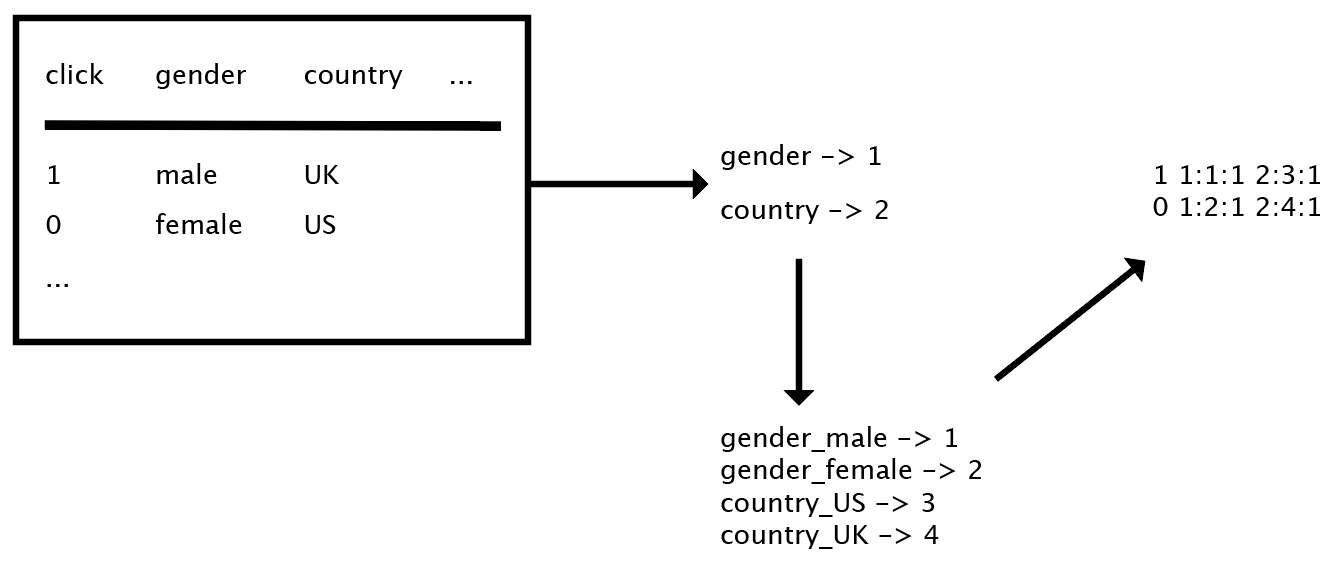
\includegraphics[width=12cm]{figures/libffm_format}}
\caption{Data format for libffm}
\end{center}
\end{figure}

The implementation provides a python interface to execute the model, loads the data into a Dato SFrame and then passes the data structure into a c++ executable, containing the model and the parameters. Unfortunately the model is known for overfitting and the results generated were not either not usable or less than that predicted by logistic regression. 

\section{Evaluation}

\subsection{Logistic Regression}

Before starting the training process of the Logistic Regression model, we first executed a hyperparameter search over ten different model configurations with the objective to get the best parameter values for the underlying data set. Table \ref{table:19} presents the results obtained during this process. Further, Table \ref{table:20} presents the iterative training progress of the Logistic Regression model, while Table \ref{table:21} presents the model's Precision, Recall, F1 score, Log Loss and AUC evaluation metrics.

\begin{table}[!htbp]
\caption{Model Hyperparameter Search for the Logistic Regression Model.}
\label{table:19}
\begin{center}
\begin{tabular}{l l l l l l}
\multicolumn{1}{c}{\bf Model ID} & \multicolumn{1}{c}{\bf L1 Penalty} & \multicolumn{1}{c}{\bf L2 Penalty} & \multicolumn{1}{c}{\bf Target} & \multicolumn{1}{c}{\bf Training Acc.} & \multicolumn{1}{c}{\bf Validation Acc.}
\\ \hline \\
9 & 100.0 & 0.0   & click & 0.999270694483 & 0.999273913501\\
8 & 100.0 & 0.0   & click & 0.999270694483 & 0.999273913501\\
1 & 0.1   & 0.001 & click & 0.999270694483 & 0.999273913501\\
0 & 0.001 & 10.0  & click & 0.999270694483 & 0.999273913501\\
3 & 0.0   & 1.0   & click & 0.99934951723  & 0.999179206566\\
2 & 1.0   & 0.01  & click & 0.999270694483 & 0.999273913501\\
5 & 0.001 & 0.01  & click & 0.999270694483 & 0.999273913501\\
4 & 100.0 & 0.1   & click & 0.999270694483 & 0.999273913501\\
7 & 0.1   & 10.0  & click & 0.999270694483 & 0.999273913501\\
6 & 100.0 & 10.0  & click & 0.999270694483 & 0.999273913501\\
\end{tabular}
\end{center}
\end{table}

\begin{table}[!htbp]
\caption{Logistic Regression Model iterative training progress.}
\label{table:20}
\begin{center}
\begin{tabular}{l l l l l}
\multicolumn{1}{c}{\bf Iterations} & \multicolumn{1}{c}{\bf Passes} & \multicolumn{1}{c}{\bf Elapsed Time} & \multicolumn{1}{c}{\bf Training Acc.} & \multicolumn{1}{c}{\bf Validation Acc.}
\\ \hline \\
1 & 2 & 8.100298   & 0.686048 & 0.685994\\
2 & 3 & 12.396830  & 0.693924 & 0.693991\\
3 & 4 & 16.601799  & 0.696544 & 0.696334\\
4 & 5 & 20.944276  & 0.697035 & 0.696948\\
5 & 6 & 25.157169  & 0.697062 & 0.696962\\
6 & 7 & 29.742889  & 0.697046 & 0.696959\\
7 & 8 & 34.197853  & 0.697046 & 0.696962\\
8 & 9 & 38.582071  & 0.697046 & 0.696959\\
9 & 10 & 42.839751 & 0.697047 & 0.696959\\
\end{tabular}
\end{center}
\end{table}

Table \ref{table:22} presents an excerpt of the ROC Curve data of the Logistic Regression Model, while Figure \ref{figure:1} showcases the ROC Curve of the Logistic Regression Model in comparison with the ROC Curve of the Boosted Gradient Machine, our two best models. The Receiver operating characteristic (ROC) Curve consists of the True and False positive rates which are used to calculate the area under the curve (AUC).

\begin{table}[!htbp]
\caption{Logistic Regression Model evaluation metrics.}
\label{table:21}
\begin{center}
\begin{tabular}{l l}
\multicolumn{1}{c}{\bf Metric} & \multicolumn{1}{c}{\bf Score}
\\ \hline \\
Precision & 0.0017458867601660326\\
Recall    & 0.7294685990338164\\
F1 Score  & 0.00348343637538064\\
Log Loss  & 0.5184005159729493\\
AUC       & 0.7961598897596291\\
\end{tabular}
\end{center}
\end{table}

GraphLab Create \cite{graphlabcreate}, the machine learning framework used in this project, consists of a parameter called \textit{class\_weights}. By default, this parameter is set to None, which means the model will only attempt to predict 0 labels as shown in Table \ref{table:23}. When set to "auto", the class weight is set "to be inversely proportional to number of examples in the training data with the given class" \cite{graphlabcreate_logistic_classifier}. In other words, the model will begin to also attempt predicting 1 labels besides 0 labels as shown in Table \ref{table:24}.

\begin{table}[!htbp]
\caption{Excerpt of the ROC Curve of the Logistic Regression Model.}
\label{table:22}
\begin{center}
\begin{tabular}{l l l l l}
\multicolumn{1}{c}{\bf Threshold} & \multicolumn{1}{c}{\bf FPR} & \multicolumn{1}{c}{\bf TPR} & \multicolumn{1}{c}{\bf P} & \multicolumn{1}{c}{\bf N}
\\ \hline \\
0.0   & 1.0            & 1.0            & 207 & 284883\\
1e-05 & 0.987545764402 & 1.0            & 207 & 284883\\
2e-05 & 0.982515629223 & 1.0            & 207 & 284883\\
3e-05 & 0.967042610475 & 1.0            & 207 & 284883\\
4e-05 & 0.947652194059 & 1.0            & 207 & 284883\\
5e-05 & 0.926878753734 & 1.0            & 207 & 284883\\
6e-05 & 0.898983091304 & 0.995169082126 & 207 & 284883\\
7e-05 & 0.882878234222 & 0.990338164251 & 207 & 284883\\
8e-05 & 0.871877226791 & 0.990338164251 & 207 & 284883\\
9e-05 & 0.860995566601 & 0.985507246377 & 207 & 284883\\
\end{tabular}
\end{center}
\end{table}

\begin{table}[!htbp]
\caption{Logistic Regression Model confusion matrix with \textit{class\_weights} parameter set to None.}
\label{table:23}
\begin{center}
\begin{tabular}{l l l}
\multicolumn{1}{c}{\bf Target Label} & \multicolumn{1}{c}{\bf Predicted Label} & \multicolumn{1}{c}{\bf Count}
\\ \hline \\
1 & 0 & 207\\
0 & 0 & 284883\\
\end{tabular}
\end{center}
\end{table}

\begin{table}[!htbp]
\caption{Logistic Regression Model confusion matrix with \textit{class\_weights} parameter set to "auto".}
\label{table:24}
\begin{center}
\begin{tabular}{l l l}
\multicolumn{1}{c}{\bf Target Label} & \multicolumn{1}{c}{\bf Predicted Label} & \multicolumn{1}{c}{\bf Count}
\\ \hline \\
1 & 0 & 56\\
1 & 1 & 151\\
0 & 0 & 198545\\
0 & 1 & 86338\\
\end{tabular}
\end{center}
\end{table}

\subsection{Boosted Tree Regression}

Before starting the training process of the GBM model, we first executed a hyperparameter search over ten different model configurations with the objective to get the best parameter values for the underlying data set. Table \ref{table:25} presents the results obtained during this process, where Model ID 9 was finally used for training, which obtained the predictions presented in Table \ref{table:26}. The \textit{class\_weights} parameter was also set to "auto" in this model.

\begin{table}[!htbp]
\caption{Model Hyperparameter Search for GBM.}
\label{table:25}
\begin{center}
\begin{tabular}{l l l l l}
\multicolumn{1}{c}{\bf Model Id} & \multicolumn{1}{c}{\bf Column Subsample} &
\multicolumn{1}{c}{\bf Max. Depth} & \multicolumn{1}{c}{\bf Max. Iterations} &
\multicolumn{1}{c}{\bf Row Subsample}
\\ \hline \\
9 & 1.0 & 8 & 10 & 0.9\\
8 & 0.8 & 8 & 10 & 1.0\\
1 & 1.0 & 6 & 100 & 1.0\\
0 & 0.9 & 4 & 100 & 1.0\\
3 & 1.0 & 6 & 100 & 0.9\\
2 & 1.0 & 6 & 10 & 0.9\\
5 & 0.9 & 6 & 100 & 0.9\\
4 & 0.9 & 6 & 50 & 0.9\\
7 & 0.9 & 6 & 10 & 0.9\\
6 & 0.9 & 4 & 50 & 1.0\\
\end{tabular}
\end{center}
\end{table}

\begin{table}[!htbp]
\caption{GBM confusion matrix.}
\label{table:26}
\begin{center}
\begin{tabular}{l l l}
\multicolumn{1}{c}{\bf Target Label} & \multicolumn{1}{c}{\bf Predicted Label} & \multicolumn{1}{c}{\bf Count}
\\ \hline \\
1 & 0 & 65\\
1 & 1 & 142\\
0 & 1 & 79665\\
0 & 0 & 205218\\
\end{tabular}
\end{center}
\end{table}

\subsection{Support Vector Machine}

We also tried implementing an SVM model to our RTB dataset, however results didn't improve our previous models. Table \ref{table:27} presents the performed hyperparameter tuning while table \ref{table:28} shows the summary of predictions on the validation set.

\begin{table}[!htbp]
\caption{Model Hyperparameter Search for SVM.}
\label{table:27}
\begin{center}
\begin{tabular}{l l}
\multicolumn{1}{c}{\bf Model ID} & \multicolumn{1}{c}{\bf Penalty}
\\ \hline \\
9 & 1.0\\
8 & 10.0\\
1 & 0.001\\
0 & 0.01\\
3 & 0.001\\
2 & 1.0\\
5 & 1.0\\
4 & 0.1\\
7 & 0.1\\
6 & 10.0\\
\end{tabular}
\end{center}
\end{table}

\begin{table}[!htbp]
\caption{SVM confusion matrix.}
\label{table:28}
\begin{center}
\begin{tabular}{l l l}
\multicolumn{1}{c}{\bf Target Label} & \multicolumn{1}{c}{\bf Predicted Label} & \multicolumn{1}{c}{\bf Count}
\\ \hline \\
1 & 0 & 58\\
1 & 1 & 149\\
0 & 1 & 82792\\
0 & 0 & 202091\\
\end{tabular}
\end{center}
\end{table}

\section{Model Comparison and Conclusion}

Figure \ref{figure:1} presents the ROC Curve and Table \ref{table:29} presents a model comparison summary of our two best models: Logistic Regression and Gradient Boosted Machine.

\begin{figure}[!htpb]
\begin{center}
\fbox{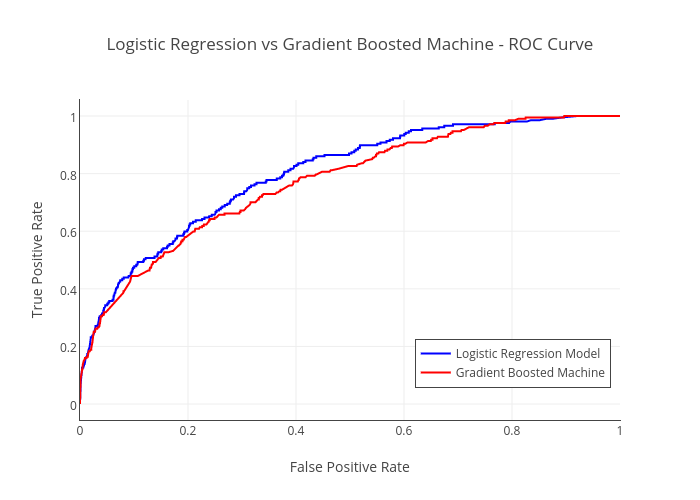
\includegraphics[width=12cm]{figures/log_gbm_roc_curve}}
\end{center}
\caption{ROC Curve of our two best models: Logistic Regression and GBM.}
\label{figure:1}
\end{figure}

Even if the GBM model obtains AUC values close to the Logistic Regression model, the former is prone to over fitting. On the other hand, the SVM model could not overcome the predictions score obtained with the first two models, but it is possible that a different set of features would boost its performance but once again, with the risk of a possible over fitting event. Our best score in the Kaggle competition is an AUC value of 0.80064 calculated against 50\% of the test set.

\begin{table}[!htpb]
\caption{Model comparison summary.}
\label{table:29}
\begin{center}
\begin{tabular}{l l l}
\multicolumn{1}{c}{\bf Model} & \multicolumn{1}{c}{\bf AUC} & \multicolumn{1}{c}{\bf Recall}
\\ \hline \\
Logistic Regression      & 0.7961598 & 0.7294685\\
Boosted Gradient Machine & 0.7718869 & 0.6618357\\
Support Vector Machine   & 0.6100004 & 0.7198068\\
\end{tabular}
\end{center}
\end{table}
\printbibliography
\end{document}